%%==================================================
%% chapter04.tex for BIT Master Thesis
%%==================================================
\chapter{系统的工具和算法原理}

本章对调度系统的区块链服务端和用户端涉及到的算法和工具进行了详细的介绍。服务器端主要涉及地理信息的存储和基于地理信息的算法工作,包括GeoHash静态矢量地图的存储,基于GeoHash静态矢量地图的路径规划算法,筛选最近的空车来与乘客进行匹配的车乘匹配算法。在车辆和乘客的用户端,主要是基于leaflet工具进行GeoHash矢量地图的展示,以及添加相应的功能来优化展示效果。

\section{基于GeoHash的矢量地图展示}

由于终端通信设备的普及和迭代,自组网系统的应用规模不断增大,基于中心化服务器的业务处理速度无法满足网络请求响应的实时性,也限制了自组网车辆之间的通信。而利用区块链的特性实现的分布式后台,既可以保证交易记录的安全性,防止恶意攻击者对地理信息和位置信息、交易信息的篡改,还可以方便成员之间的相互通信,同时其分布式的特性也能够满足对大规模网络请求的及时响应。

本节将介绍GeoHash矢量地图在区块链中的存储逻辑,同时还会介绍在终端页面实现的对GeoHash矢量地图的渲染逻辑,以及为了优化地图展示效果补充的放缩和拖动功能的实现逻辑。

\subsection{基于GeoHash的地图在区块链上的存储}

GeoHash是一种新型的地址编码方式,由Gustavo Niemeyer和G.M. Morton发明[董斌37],其具体算法是二分法结合编码的一种地理位置信息算法[董斌16],被广泛应用到地理位置表示中。最开始,以本初子午线、赤道为界,地球可以分为 4 个部分,设定西经为负,南纬为负,所以地球上的经度范围就是 [-180,180],纬度范围就是 [-90,90]。GeoHash 使用了Peano空间填充曲线\ref{fig:peano},在处理地图数据的过程中,要将经纬度点转换成GeoHash,首先要通过二分的方法把经纬度转化成二进制编码,

% 以 (116.3639092,39.9662639) 为例,将其转化为精度为8位的GeoHash,过程如下表3-1所示(一张表用来示例)。

将经度和纬度分别转换成一组二进制字符串,然后将经度和纬度的二进制字符串以位置交叉的形式进行组码,生成一组新的更长的二进制字符串,新的二进制字符串中偶数位的数字对应原来的经度二进制串,奇数位的数字对应原来的纬度二进制串,然后将新二进制串每五位一组,转为十进制数字,并根据数字找到其在Base32(即数字 0-9 和字母 b-z 不包括 a,i,l,o 的 32 个字符) 数组的映射,以此进行编码[董斌16],最终实现用GeoHash一维数据表示原经纬度二维数据的效果。

\begin{figure}
  \centering
  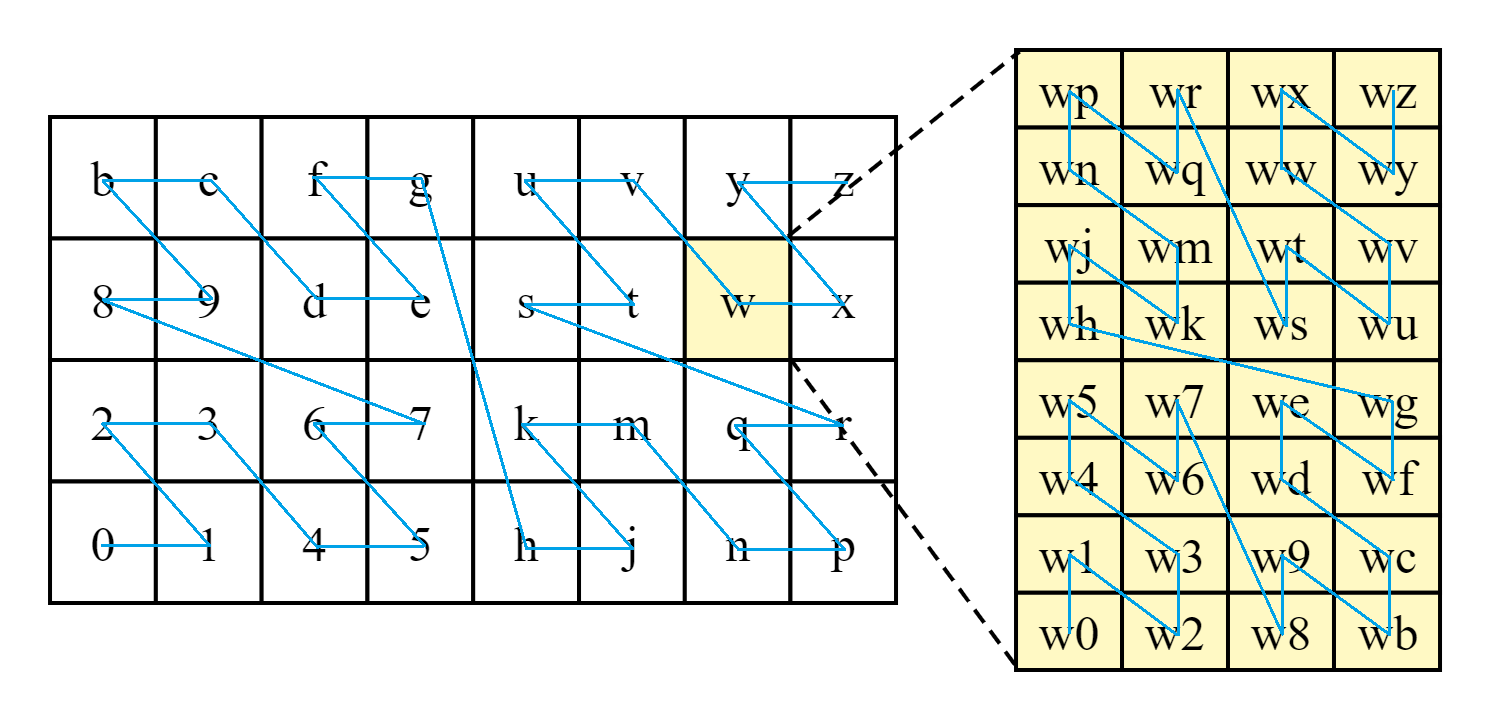
\includegraphics[width=1.0\textwidth]{figures/peano}
  \caption{GeoHash划分和Peano曲线示意图}\label{fig:peano}
\end{figure}


根据Geohash特殊的编码方式,一个GeoHash值对应一个近似矩形的覆盖区域,当位数较短时,它可以表示一块区域的位置,当位数足够长时,它可以表示地球上某个具体点的坐标,重要的一点是,GeoHash位数短的区域一定包含以这个GeoHash为前缀的所有地图数据,如图\ref{fig:fatherAndSon}所示,这一特点对地图数据进行区域绑定提供了极大的便利。GeoHash在编码过程中保留了一定的相对地理位置信息,在大部分情况下,GeoHash编码共同前缀越长的区域相距越近[董斌37],一个6位GeoHash块的覆盖区域大小为1220m*1220m。

\begin{figure}
  \centering
  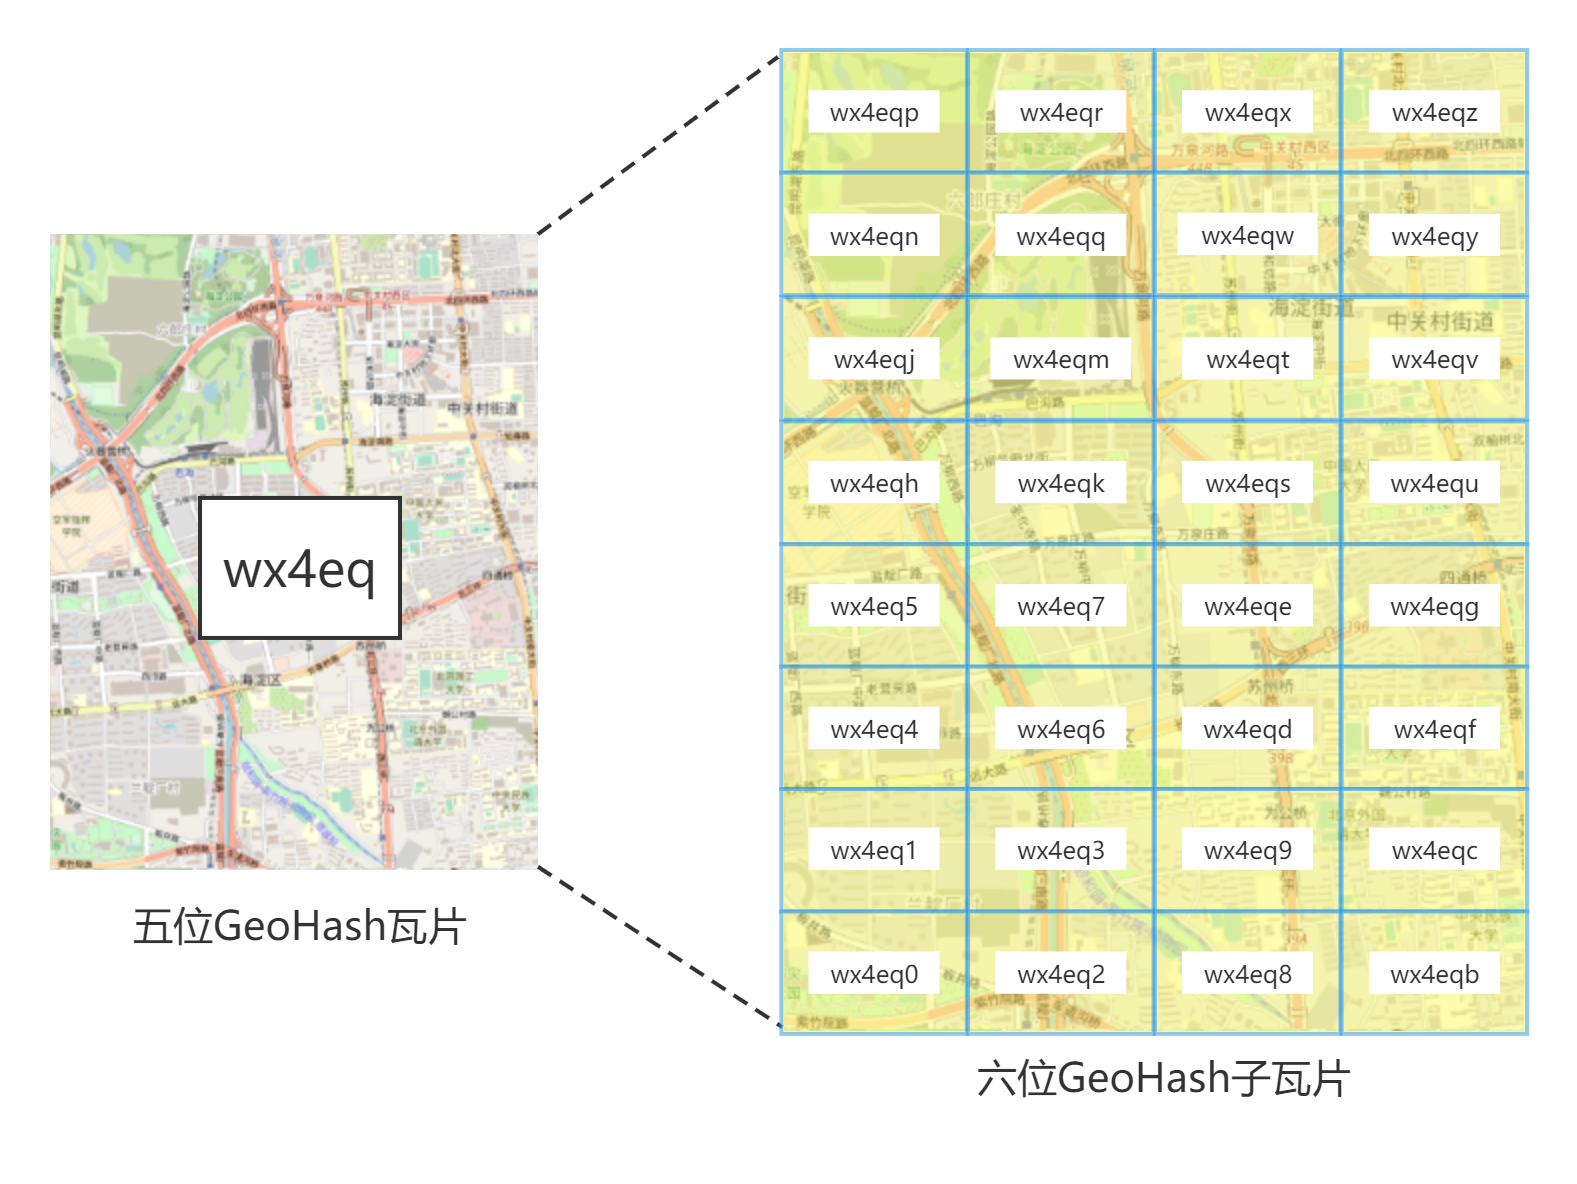
\includegraphics[width=1.0\textwidth]{figures/瓦片与子瓦片}
  \caption{GeoHashTile瓦片与子瓦片的包含关系}\label{fig:fatherAndSon}
\end{figure}


传统的地图数据采用经纬度的方法进行存储,不方便实现位置与区域绑定,并且二维数据存储内容较大,对网络环境和存储设备的要求较高。采用 GeoHash 字符串存储地图信息可以使所有信息平面化,更方便区域信息绑定,并且一维字符串降低了存储数据的规模,同时基于GeoHash地理信息的运算复杂度较低,也更适用于 Solidity 语言。

车辆和乘客的终端在使用时需要从区块链中读取地图信息。为了降低地图数据对终端设备的内存要求,以及降低对网络资源的占用,在区块链存储地图时可将地图进行分块处理,这样终端不用一次读入所有的地图信息。同时,分块后的道路会按照其GeoHash位置的前缀绑定到相应的GeoHash区域内,这样终端在获取地图时能够根据用户的GeoHash位置读入该GeoHash所属的大范围GeoHash区域的地图信息,而不用遍历所有的地图数据,在提高获取效率的同时还会减少网页端的内存消耗,也便于终端地图信息的更新。
% (一张区域绑定示意图)

智能合约中存储的道路信息包括道路ID、道路起点位置、终点位置、道路路径上的点构成的数组(道路为折线段结构)、标识道路间连接信息的 ID(每条道路只在首尾处与其他道路相接)、道路名、道路长度以及单双向行驶标识如表\ref{tab:roadFormat}所示。道路信息属于静态数据,在存储到地图合约的过程中,会对道路末尾连接处所能到达的所有道路的信息记录成一个数组,以方便路径规划算法在运行时对下一条可达道路的启发式查找(记录的算法)。另外,由于开发语言不支持浮点数,因此距离信息需要用GeoHash距离运算的整数结果来表示,此处需要调整运算过程中的参数来找到准确度和运算效率双优的参数。
% (一张参数表)

\begin{table}
  \centering
  \caption{GeoHash道路数据格式}\label{tab:roadFormat}
  \begin{tabular*}{0.9\textwidth}{@{\extracolsep{\fill}}cccc}
  \toprule
    编号    &字段名称 &字段类型 &字段含义 \\
  \midrule
    1    &gid &int &道路id\\
    2    &name &string &道路名称\\
    3    &highway &string &道路类型\\
    4    &cost &int &道路长度(米)\\
    5    &sourceGeoHash &string &道路起点位置\\
    6    &targetGeoHash &string &道路终点位置\\
    7    &source &int &道路起始点的id\\
    8    &target &int &道路终止点的id\\
    9    &oneway &int &道路是否是双向的\\
    10    &coordinates &arraylist &道路路径经过的点\\
  \bottomrule
  \end{tabular*}
\end{table}

\subsection{基于GeoHash的矢量地图的终端数据显示}
画一个流程图,按流程图描述(一图)
1.计算当前层级GeoHashTile的size
2.计算当前屏幕内GeoHashTile的个数(一共5个公式)
3.计算当前屏幕内所有GeoHashTile的编码(简单提及)
4.向服务端请求地图数据(简单提合并的过程)
5.压缩数据,计算GeoHashTile的中心GeoHash(简单提)
6.计算像素距离(简单提及)
7.计算地图对象的屏幕坐标(1个公式)
8.将tile pixel distance和coordinate pixel distance做缓存(简单提及)

[周畅]的GeoHashTile工作设计了基于GeoHash体系的矢量地理数据结构——GeoHashTile,利用了GeoHash对矢量地理数据的高效分区和一维索引,方便对地理数据的查询,并且其支持了对GeoHash地理信息的显示,实现了GeoHash坐标和屏幕上像素坐标的直接转换,并且验证了GeoHashTile在请求数据的速度上比基于经纬度的GeoTile系统有明显优势。其GeoHash转换成屏幕坐标采用的是相对投影的方法。

终端完成显示Geohash矢量地理数据的过程,如图5所示,主要包括三个部分:
(1)计算GeohashTile的数量和编码,包括三个步骤:首先获得当前缩放级别下一块GeohashTile的像素大小(每个级别的瓦片像素大小已经通过推理计算设置好[周畅论文]),然后通过屏幕的长宽像素计算客户端中GeohashTile的数量,得到数量后,再通过中心瓦片的GeoHash编码和查找邻居瓦片的算法,计算终端屏幕中所有GeohashTile的编码。
(2)地图数据请求发送到服务端之前,为了减少请求报文的规模,使用GeohashTile请求合并算法来实现要发送的请求的合并。服务器收到请求后会查找请求的所有区域的数据,并整理成基于GeoHash的GeoJSON数据返回给终端。
(3)终端收到地图数据后会进行投影显示,相对位置投影过程包括数据压缩、计算像素距离和计算屏幕坐标三个步骤。实现投影的第一步是计算从这些目标点到中心点的相对像素距离列表。有两种相对距离计算(如图5中的步骤6所示)。第一个是计算从各个GeohashTile中心像素点到屏幕中心像素点的相对像素距离。第二个是计算从目标点的像素点到其所属GeohashTile中心像素点的相对像素距离。将这二者相加即可得到目标点的在屏幕中的像素位置,通过画点接口进行投影。

% 4.1.1. 计算一块GeohashTile的大小,如步骤1所示?如图5所示。在瓦片地图系统中,瓦片的索引遵循四叉树原则。在每个缩放级别,等式(2)用于计算在x轴和y轴方向上的瓦片数量,其中z是缩放级别。
% 公式(2)
% Geohash编码的每多一个字符就代表将一块区域进行更深层的子分区,一个区域根据编码的奇偶字节交替划分为4×8或8×4子区域。每次分区后对应的x轴和y轴方向上的GeohashTile编码数量的计算公式为公式(3),其中l是Geohash编码的长度。 
% 公式(3)
% GeoHashTile的缩放级别z与GeoHash的字符长度l并不是严格相关的。由于GeoHash每一层的分区都多于GeoTile系统中的四叉树分区,因此,我们结合方程(2)和(3)得到Geohash编码长度l和缩放级别z之间关系的方程(4),在满足公式(4)的基础上,使用最短长度的Geohash编码来做瓦片,以减少存储。对于每个层级z,l的计算结果取最小整数。
% 公式(4)
% 无论谷歌地图、必应地图或其他地理信息显示系统如何,每层的分幅都是固定的像素大小(最常见的分幅像素大小为256×256)。从上面可以看出,Geohash每一层的瓦片大小都是相同的,并且层与层之间的瓦片大小根据划分规则有规律地变化。由于x和y方向的分割大小不一致,Geohash瓦片大多为矩形。为了使GeohashTile在每个级别上近似于256×256的平方像素大小,并便于计算,GeohashTile的像素大小在缩放级别0设置为512×512。结合方程式(4)的计算结果,可通过方程式(5)计算相应缩放级别z下的GeohashTile大小。在等式(5)中,z是缩放级别,l是Geohash编码长度。由于Geohash在x和y方向上的除法规则不一致,因此需要两个不同的方程来完成计算。 
% 公式(5)
% 表3显示了通过等式(5)计算的GeohashTile的像素大小,其中缩放级别为1–18。除了能够计算具有不同编码长度的GeohashTile的像素大小之外,等式(5)还用于稍后计算Geohash坐标点转换屏幕像素坐标。
% 表3
% 4.1.2. 计算客户端中GeohashTile的数量在获得相应缩放级别中GeohashTile的大小后,可以通过组合客户端像素大小来计算屏幕中覆盖的GeohashTile的数量,以便为从服务器获取相应的地图数据做准备(如图5中的步骤2所示)。方程式(6)是计算地砖坐标x轴和Y轴方向上的GeohashTile编码数量的方程式,其中大小为。x、 尺寸。y是客户端屏幕的像素大小。
% 公式(6)
% 为了确保GeohashTile覆盖屏幕,计算结果将被四舍五入。这也是图5所示GeohashTile覆盖范围超出屏幕的原因。

% 4.1.3. 计算客户端中的所有GeohashTile编码以从服务器获得相应的地图数据,我们应该计算屏幕覆盖范围中的所有GeohashTile编码(如图5中的步骤3所示)。

% 4.3 相对位置投影处理所有地图数据都需要从球面数据投影到二维平面数据进行显示。本节描述的Geohash地图数据的相对位置投影过程是使用相对位置计算方法将Geohash编码的地图数据直接投影到屏幕坐标的过程。具体计算步骤如下:

% 4.3.1. 编码长度和缩放级别的关系
% 公式(7)
% 公式(8)
% 这里我们有两个定义来帮助解释。
% 定义1
% 定义2
% 公式(9)
% 4.3.2. 计算相对像素距离
% 算法3

% 4.3.3. 客户端屏幕中心点像素+tile中心点像素偏移+coord相对tile中心点的偏移

\subsection{基于GeoHash的矢量地图实现放缩和拖动功能}

上一节主要讨论了GeoHash矢量地理数据在终端的的投影过程,其核心工作是将GeoHash字符串转投影为屏幕上的像素坐标。本节讲述实现放缩和拖动功能的原理工作,其核心部分的实现逻辑与上一节所述内容相反,实现放缩和拖动功能需要重新设置地图视野的中心点GeoHash,这需要将鼠标在屏幕上的像素点位置转化成相对应地图图层的GeoHash地理位置。(逻辑流程图)

实现GeoHashTile的拖动功能,即通过监听终端操作获得给定的像素值变化,然后对地图进行平移;实现放缩功能,即通过监听终端操作获得缩放等级的变化,然后将地图展示成新的缩放等级。放缩或者拖动结束之后,需要重新获取视野的中心点GeoHash字符串,这个工作是将变化后的地图图层的中心点投影成GeoHash字符串,需要实现将屏幕的像素坐标投影成GeoHash字符串的功能。

首先遍历屏幕内的所有GeoHashTile瓦片,通过(算法1)根据每个瓦片的范围判断操作点所在的瓦片,然后获得该瓦片的中心点GeoHash和中心点像素位置,通过操作点的像素位置和操作点所在的GeoHashTile的像素位置,可以通过(公式1)计算出两点之间的相对像素差,根据相对像素差,结合本缩放层级下的瓦片像素大小,可以通过(公式2)计算出操作点和瓦片中心点在该精度下的GeoHash在东西和南北方向上的地理偏移量(以瓦片中心点GeoHash的精度下所对应的GeoHash格子数表示),根据操作点相对于瓦片中心点的GeoHash地理偏移量,可以通过(算法2)计算出操作点的GeoHash,此GeoHash的精度与瓦片中心点GeoHash相同。(放大缩小示意图)

7086_onDragEnd->map.panBy(offset)将地图按给定像素平移

\section{基于GeoHash的几何计算优化}
由于传统计算两个经纬度所表示坐标点距离时需要使用球面距离公式,若在以 GeoHash 为坐标表示的系统中沿用这套算法,则丧失了 GeoHash 带来的计算简便性。利用GeoHash编码的特点进行距离计算,避免了复杂的三角函数和球面计算,并且适用于对小数支持较弱、不提供复杂数学函数计算支持的区块链智能合约编写语言 Solidity。

\subsection{GeoHash几何计算原理}

在将经纬度编码为GeoHash时,首先要将经纬度分别通过二分法编码为对应长度的二进制编码,然后将经度和纬度的二进制编码按照偶数位放经度的二进制编码、奇数位放维度的二进制码的方式进行组码,最后将新获得的组码串进行Base32编码,即可获得GeoHash字符串。

在上述编码的过程中,经纬度二分后对应的两个二进制编码,其对应的十进制值也有特殊的地理意义:即在当前要编码的GeoHash精度下,这一对经纬度对应的GeoHash瓦片,相对于地球原点处所偏移的相同规模的GeoHash瓦片的数量。经度对应的二进制编码的十进制值表示在东西方向上偏移的瓦片数量,纬度对应的二进制编码的十进制值表示在南北方向上偏移的瓦片数量。

根据上述原理,在计算两个GeoHash位置之间的距离时,可以先将两个GeoHash各自解码为在东西和南北方向上表示偏移的数值,再计算这两者在东西和南北方向上偏移的数值之差,即可得到两点之间在东西和南北方向上的相对位置差。由于经纬度划分的原因,在一定的GeoHash精度下,所有瓦片的南北距离都是相同的,但东西距离会根据GeoHash点所在纬度的增加而减小。在10位GeoHash精度下,每个瓦片的东西宽度,可以按纬度的不同大致划分为16个区域。故两个GeoHash点之间的南北距离可以根据南北瓦片的偏差值乘以当前GeoHash精度下瓦片的南北距离(单位:米)获得;而两个GeoHash点之间的东西距离需要根据GeoHash所属的纬度区域找到GeoHash瓦片的东西距离(单位:米),再乘以两者的东西瓦片偏差值获得。

\subsection{GeoHash几何计算方法的优化}
在实际的出租车系统应用环境中,两个终端之间的距离计算所涉及到的地区范围,通常情况下不会超过市辖区以上的规模。故在出租车系统的环境下,两个终端的地理位置GeoHash会有一定位数的前缀是相同的(通常在5位到6位,见表\ref{tab:GeoHashScale})。据此,这两个GeoHash解码后的二进制偏移值的前几位也会相同。事实上二者相同前缀所转化的高位数字是相同的,做减法之后会相互抵消。这些相同前缀转化的的高位数字对二者相对偏移的计算没有影响,这就造成了在GeoHash解码时对计算资源的浪费。

\begin{table}
  \centering
  \caption{GeoHash的长度和距离精度的关系}\label{tab:GeoHashScale}
  \begin{tabular*}{0.9\textwidth}{@{\extracolsep{\fill}}cccc}
  \toprule
    GeoHash长度    &纬度偏差 &经度偏差 &距离偏差(km) \\
  \midrule
    1    &$\pm23$ &$\pm23$ &$\pm2500$\\
    2    &$\pm2.8$ &$\pm5.6$ &$\pm630$\\
    3    &$\pm0.70$ &$\pm0.7$ &$\pm78$\\
    4    &$\pm0.087$ &$\pm0.18$ &$\pm20$\\
    5    &$\pm0.022$ &$\pm0.022$ &$\pm2.4$\\
    6    &$\pm0.0027$ &$\pm0.0055$ &$\pm0.61$\\
    7    &$\pm0.00068$ &$\pm0.00068$ &$\pm0.076$\\
    8    &$\pm0.000085$ &$\pm0.00017$ &$\pm0.019$\\
    9    &$\pm0.000021$ &$\pm0.000021$ &$\pm0.0024$\\
    10    &$\pm0.0000027$ &$\pm0.0000055$ &$\pm0.00060$\\
    11    &$\pm0.00000067$ &$\pm0.00000067$ &$\pm0.000075$\\
  \bottomrule
  \end{tabular*}
\end{table}

在地理视角上,计算两个GeoHash之间的距离,首先是对GeoHash进行解码计算出二者相对地球原点的偏移,如果计算时排除掉两个GeoHash前缀相同的部分,如图\ref{fig:calBetter}所示,此处的参照对象就会从地球原点改为同时包含这两个GeoHash瓦片前缀瓦片(即二者相同前缀部分的GeoHash所表示的瓦片)原点,以距离二者更近的原点作为参照,可以减少计算瓦片偏移数量时的运算规模,从而加快运算速度,使距离计算的算法性能得到提升。

\begin{figure}
  \centering
  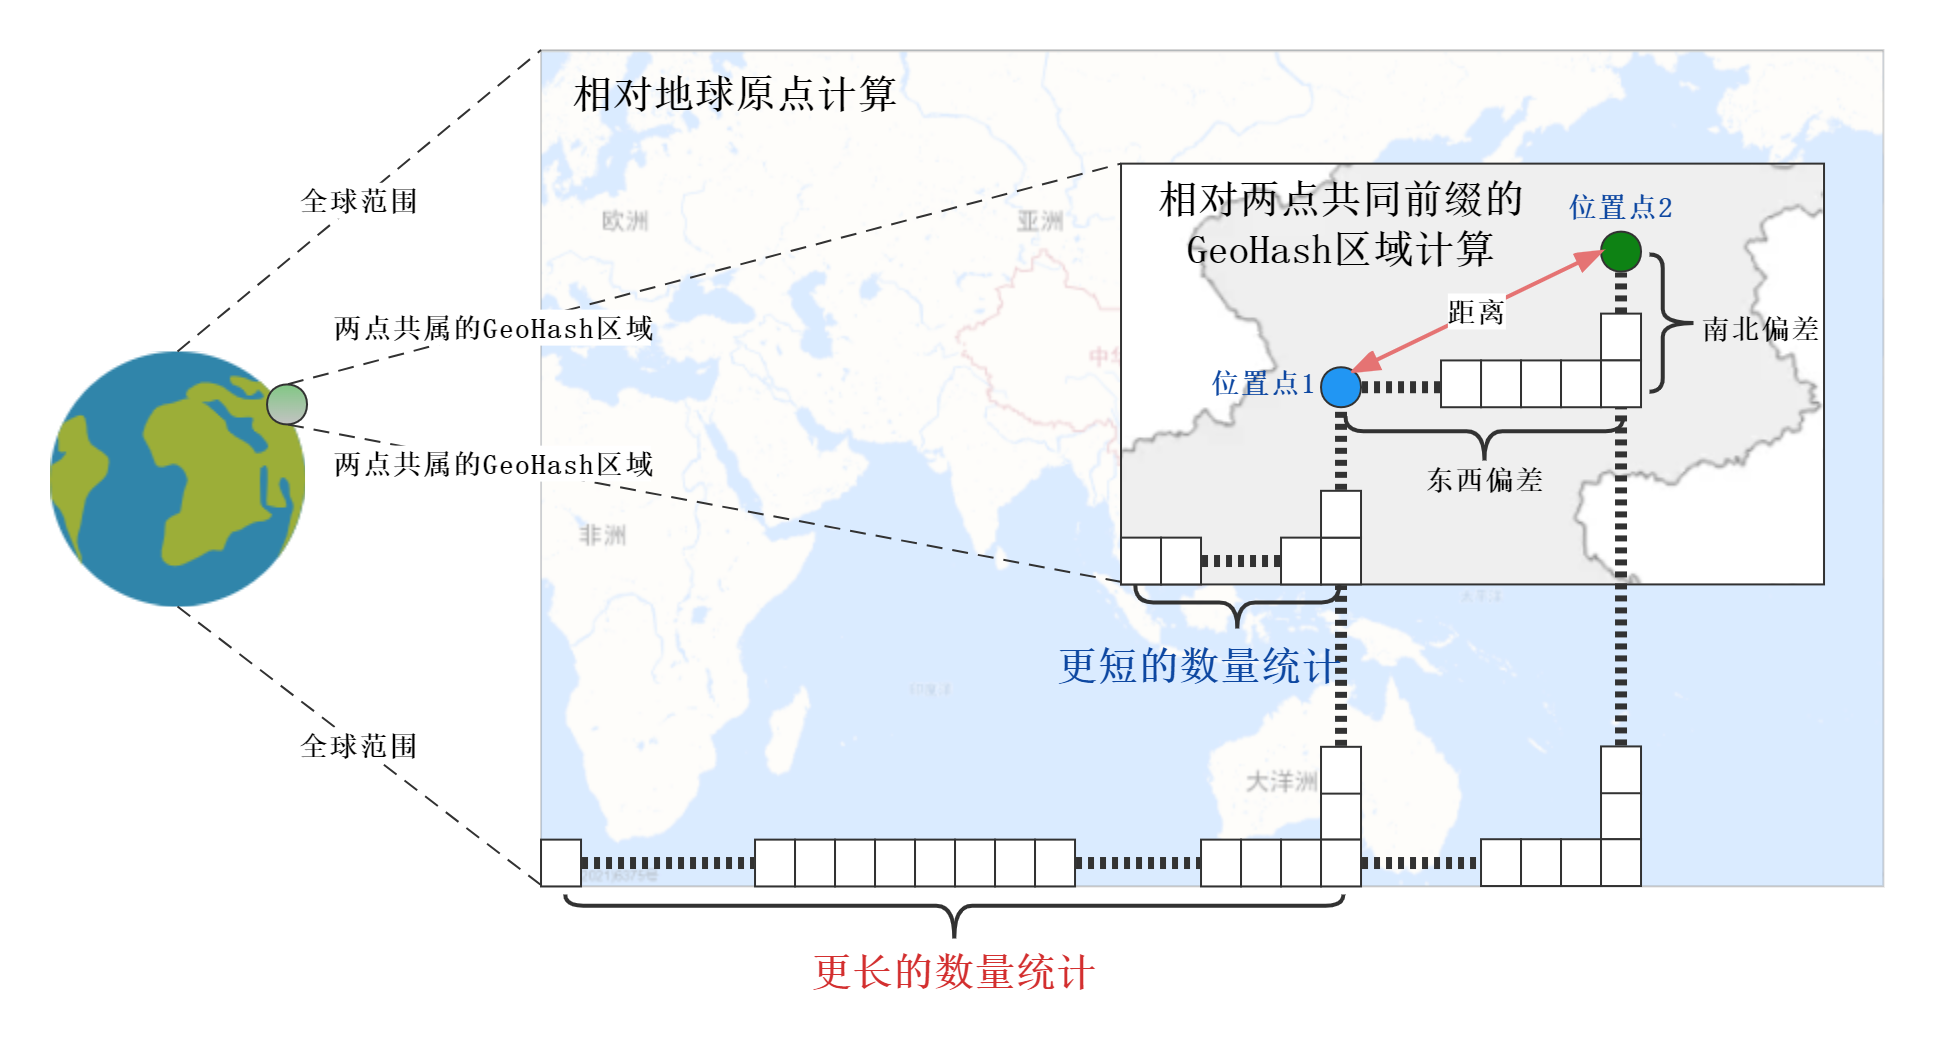
\includegraphics[width=1.0\textwidth]{figures/GeoHash计算优化}
  \caption{GeoHash几何计算优化示意}\label{fig:calBetter}
\end{figure}

本文在进行GeoHash距离计算时,首先检查两个GeoHash的前缀相同的部分,然后取其不同的部分进行距离计算,以优化距离计算的性能,利用了GeoHash字符串的特性,加快系统的响应速度。在智能合约中的算法的逻辑如算法\ref{alg:shortGeoHash}所示,具体的性能优化效果在第五章进行描述。

\begin{algorithm}[t]
  \caption{相同前缀的优化过程算法}
  \label{alg:shortGeoHash}
  \begin{algorithmic}[1]
  \REQUIRE input parameters $geohash1$, $geohash2$
  \ENSURE output $shortGeo1$, $shortGeo2$
  \STATE PRECISION = geohash1.length;
  \FOR{index = 0; index < geohash1.length; index++}
    \IF{geohash1[index] != geohash2[index]}
      \STATE break
    \ENDIF
  \ENDFOR
  \STATE dif = PRECISION - index
  \STATE index2 = 0
  \FOR{j = index; j < PRECISION; j++}
    \STATE shortGeo1[index2] = geo1[j];
    \STATE shortGeo2[index2] = geo2[j];
    \STATE index2++;
  \ENDFOR
  \RETURN shortGeo1, shortGeo2
  \end{algorithmic}
\end{algorithm}

\section{基于GeoHash的路径规划算法}
为了完善去中心化的出租车调度系统,需要在智能合约端实现后台的路径规划算法。路径规划算法的提出和发展由来已久,有适合在未知地图环境下运行的启发式路径规划算法,可以应用在智能机器人和无人车等领域,如机器人的自动寻路、游戏中的AI角色寻路等场景。此外,还有可以在已知地图信息的情况下,利用已有的矢量地图数据规划出最短路径的算法,可以应用在地理信息实时更新的交通系统中,如车载应用的路径规划、公共交通实时路径规划等环境。

本文所描述的系统已有静态矢量地图拓扑信息的支持,故采用静态路网的路径规划算法为车辆提供路径规划的辅助。路径规划算法需要根据智能合约上存储的GeoHash矢量地图数据进行静态导航,参考GeoHash地图存储的格式,在进行地图存储时根据路口的连接关系建立路口之间的拓扑连接关系。本节采用优化后的GeoHash距离计算方法,结合常规静态路网规划算法A*算法,提出了基于GeoHash矢量地图的路径规划算法,为车辆提供路径规划服务。本节实现的路径规划算法可以根据不同的道路权值类型进行路径规划,还可以调节算法参数,在保证路径规划准确性的前提下提高效率。同时,为避免不必要的服务纠纷,会对路径规划的结果进行记录。

\subsection{矢量地图路径路径规划算法的对比选择}

Dijkstra算法是由E.W.Dijkstra于1959年提出,属于贪心算法模式,是非常典型的最短路径算法。此算法可以用于求得移动机器人行进路线中的一个节点到其他所有节点的最短路径。算法的主要特点是:以输入的起始点为中心,算法过程中生成无向图一直向外扩展,直到扩展到最终的目标点为止,通过节点和权值边的连接关系来构成整个路径。Dijkstra算法的缺点是效率低,在无向图扩展的过程中会生成大量的无效路径,占用较多的内存空间。

A*算法(Dijkstra with a Heuristic)是在Dijksra的基础上加入启发式函数实现的,因为加入启发算子的缘故,在拓展无向图的过程中可以根据目标点相对中间点的距离协调选择最好的方向进行搜索。相比Dijkstra算法的效率更高,占用内存空间更少。A*算法的应用范围比较广,可以在电子地图进行路径规划,或者在游戏领域中应用于虚拟角色的行走路径的规划,A*算法的计算结果正确性较高,能够调整算子来适应不同的路径权值类型,拓展了其健壮性和适用范围。

JPS算法在A*算法框架的基础上加入了跳点搜索(Jump Point Search),JPS会根据当前点的方向及当前点周围邻居的特点进行选择,某些特殊的点才能执行加入和删除到可探索点集合的操作。在网格地图中,JPS算法可以用来提高有障碍物时的寻路效率,在遇到障碍物时需要改变搜索方向,这时只把能够以最短路径避过障碍的跳跃点加入可探索点集合中,可以避免考虑很多不必要的路径点,以此来提高算法的搜索效率。但本文的静态地图在储存时已经生成邻居道路的拓扑结构,不需要考虑避开障碍物。JPS算法在已有拓扑结构的地图中徒增算法的复杂度,故不在本文应用。

CH算法在A*算法的基础上加入了预处理的过程,算法在预处理阶段创建“shortcuts”来实现提速,然后在最短路径查询中使用这些“shortcuts”来跳过“不重要的”顶点。“shortcuts”可用于保存两个重要路口之间预先计算的距离,从而算法无需在查询时考虑这些路口之间的完整路径,这样可以使查询路径缩短,查询效率得到提高。但CH算法的预处理使得查询时的道路网络失去了真实的拓扑结构,在每一条道路信息更新后都需要重新对全局进行预处理;此外,道路权值类型的更改也会重新触发整个预处理过程,不能很好地支持实时的交通信息,系统的拓展性和健壮性不足。

\subsection{基于GeoHash的A*路径规划算法的原理}
A*算法是一种直接查询算法,只需要地图的拓扑数据,而不需要做任何预处理。同时 A*算法是一个启发式算法,利用了启发函数,A*算法的启发函数算子可以记成 h(n),代表着算法过程查询到的中间节点到目的地节点的距离估计值。A*算法在选择路径中第n个被检查的节点时,还会参考从起始点到第n个中间节点的实际距离,称为耗散函数,记为 g(n)。A*算法的对中间节点的估计函数(如公式\ref{eqn:calCost})同时参考了耗散函数和启发函数,将二者的和作为评价该节点处于最优路线上的可能性的量度,这样可以首先搜索可能性大的节点。在算法运行的过程中,A*算法根据评估函数f(n)的值,找到距离终点最近的可能性最大的节点,然后展开搜索该节点,而不用每一步规划都需要搜索所有节点,提高了路径规划的效率。

\begin{equation}
  \label{eqn:calCost}
  f(n)=g(n)+h(n)
\end{equation}

A*算法的的核心是设置一个合适的评估函数,评估函数的计算方式对搜索结果有决定性作用。对第n个中间节点来说, g(n) 的值基本是固定的,其反映的是从起点到当前节点的实际道路距离。因此,启发函数 h(n)的选择就显得更重要,它能控制 A*算法计算过程中的行为。如果把 h(n)设置为 0,这时候 f(n)=g(n),A*算法就会退化为 Dijkstra 算法,也能计算出目标路径。启发函数的影响越小,在 A*寻路时需要探索的节点越多,寻路过程就会变慢。启发函数 h(n) 的值如果设置的比 g(n) 大非常多,相当于只有启发函数起作用,A*算法接近 BFS 算法,路径规划的结果不一定是最短路径。
常用的启发函数 h(n)二维坐标下有以下几个距离度量方法:
(1)曼哈顿距离,表示在标准坐标系上的绝对坐标轴距之和,(公式)

(2)欧几里得距离,也叫欧式距离,表示两点之间的直线距离。(公式)

本文的实验部分基于GeoHash矢量地图数据,道路属性里的cost字段记录的是道路的实际长度,这个长度即是每条路段的两个端点之间的距离,以米为单位。为了简化启发函数的计算,从而支持智能合约语言的特性,本文采用曼哈顿距离作为度量,结合GeoHash计算距离的函数进行启发函数的计算。为了使启发函数 h(n) 的结果与实际情况更接近,本文调整了GeoHash计算距离函数的参数,使启发函数的结果更接近真实的道路距离,这一步可以让路径规划结果的正确性和算法的效率都得到保障。


\section{基于树状区块链的区域调度车乘匹配算法}1段

在本文的系统中,车辆和用户在初始化自己的信息时,会在智能合约端注册自己的身份和位置信息,智能合约会按照注册的先后顺序对车辆和乘客的信息分别进行记录。在乘客发出乘车请求后,智能合约开始根据乘客的位置来为乘客匹配到最近的空车。在查询空车时,需要按车辆注册的顺序遍历每一辆车,同时查询车辆的载客状态和车辆相距乘客的距离,寻找到距离乘客最近的空载车辆,然后将乘客的请求发送到这辆车的终端,车辆根据乘客的起止点位置来判断是否执行订单。

但是对于大规模应用的系统来书,按注册先后顺序遍历车辆信息的方法显然是低效的,在遍历过程中会查询到较多距离乘客位置较远的车辆,属于无效查询,浪费计算资源,同时也没有利用好分布式系统的特点。树状区块链[周畅论文]将地理信息融合到区块链的分布式系统中,可以根据地理区域快速查询在特定地理区域里的账户信息。故相比传统区块链,融合了地理信息特性的树状区块链能够更好地支持本系统的车辆调度分配工作。

\subsection{树状区块链对区域信息的查询}4-6段
介绍树状区块链对区域信息的查询原理。

区块链结构
如图2-1,树状区块链是基于以太坊的区块链数据结构进行修改的,在其基础上主要新增如下数据结构:
(a) 同层块指针:记录与本区块同层次地理区域对应区块的哈希,与父块哈希一同构成树状区块链。
(b) 位置:使用指定长度的 Geohash 编码表示位置,分别在账户状态、交易数据中新增位置信息,增加账户、交易与物理世界的关联。
(c) 区域状态树:以 Geohash 作为索引构建字典树,存储区域内的四种信息:当前区域内的账户(Account)、交易(TXID)、收据(RPID)以及上层区域状态树根节点列表(URRList)记录所有上层区域状态树的根节点哈希,如图2-2。
(d) 账户位置树:记录账户发生过的交易所在的区域。可以提供以下功能:根据位置区域,查询该区域内最新交易;查询某个账户在指定区域的交易以及历史交易发生的位置, 如图2-3。

区块与节点的层次化分类
为了将区块链划分为树状结构,首先将区块按其特征分为三种:
(a) 创世块:区块链的初始区块。
(b) 分支块:根据 Geohash 编码以层次化结构一一对应创建分支区块作为对应区域内子链的头区块,只维护直接下层区域的索引信息,不记录交易信息。
(c) 普通块:地理区域的最小划分对应分支区块的子区块,记录在对应地理区域内发生的交易。其次,将网络节点按照其功能分为三种:
(a) 全节点:维护全区块链完整区块数据和全局状态树,部分服务器为全节点。

(b) 区域节点:维护其所在区域内指定层次及以下的所有分支区块与普通区块。每个分支节点负责向上层节点更新汇总当前区域状态并同步所有上层区块链的区域状态树根节点列表。路侧节点与部分服务器为区域节点。
(c) 叶节点:维护所在区域内最下层分支区块以及普通区块。负责局部共识,以及在与区域节点有连接机会时上传缓存信息,并同步所有上层区块链的区域状态树根节点列表。车辆节点为叶节点。
3. 区块的层次化组织
在树状区块链设计中,只有普通区块会记录实际发生的交易,分支区块提供子区区块链头区块以及索引功能。每个地理区域都有对应一个分支区块和多个普通区块通过父块哈希指针组成的区块链,同层次不同区域中的分支区块之间通过同层块指针链接起来。分支区块的层次关系代表地理区域的包含关系,即上层分支区块对应的地理区域包含所有以该区块为父块的下层区块对应的地理区域。
树状区块链与传统区块链相比,融合了地理位置,设计了区块状态树和账户位置树等与地理位置相关的数据结构,增加了区块链与真实世界的联系,提升与地理信息相关数据的检索速度。

\subsection{区域调度车乘匹配算法}3段
介绍在树状区块链对区域信息查询的基础上实现的区域调度车乘匹配算法原理、对并发请求的冲突解决逻辑。

利用树状区块链区域查询的特点,可以快速获得区域内的车辆账户信息。当乘客发出乘车请求后,智能合约会根据乘客的位置从树状区块链获得乘客所在区域内的车辆列表,然后根据最近匹配空车的原则从区域的车辆列表中找到最合适的车辆。考虑到区域范围的大小,5位长度的GeoHash所代表的范围是()米*()米,而6位GeoHash所代表的范围是()米*()米,如果考虑的区域范围过大,则涉及到的车辆数量会显著增加,在一定程度上也影响了匹配的速度;如果考虑的范围区域太小,则可能无法找到合适的车辆。

综合上述问题的考虑,结合树状区块链区域查询的优势,本文提出了基于GeoHash邻居查找的区域调度算法,具体算法过程(如图)所示,系统根据乘客的上车点位置的GeoHash,直接取GeoHash字符串的前缀,可以找到乘客所在位置的GeoHash区域,再根据GeoHash查找邻居的算法找到乘客所在区域以及其周围八个区域共九个区域的GeoHash,从树状区块链的区域状态查询中找到在这些GeoHash范围内的所有车辆信息,然后智能合约会从这些车辆中找到距离最近的空车作为匹配结果。

在智能合约评估每辆车和乘客的距离时,如果只通过车辆和乘客的GeoHash位置相同的前缀个数来判断距离,由于GeoHash代表的范围随其长度的变化较大,无法对各个车辆的远近做有效的区分,而且(论文)提出的方法没有考虑到GeoHash的边缘效应(示意图),无法准确反映车辆和乘客的实际距离。故本系统在评估车辆和乘客距离时采用基于GeoHash的距离计算方法,可以通过调节参数在不同规模的GeoHash大小上统计车辆和乘客的距离,可以通过实验选取合适的参数,既保证匹配结果的准确性,也保证计算过程的高效性。

本文的区域调度方式可以有效提高车乘匹配的效率,且同时保证了车乘匹配的就近原则,合理地满足了乘客的乘车需求;同时还利用了树状区块链的地理信息特性,通过第五章的实验部分评估了区域调度的正确性和高效性,用实际的应用和实验验证了将区块链与地理信息相结合的技术优势。

\upcite{2016A}考虑正常交通对出租车的影响,提出了一种出租车调度系统,该系统使用实时交通状况将空置的出租车与最近的(在旅行时间方面)等候的乘客相匹配。